
\documentclass[8pt]{beamer}
\usepackage[authoryear,round]{natbib}
\usepackage{graphicx}
\usepackage{fancybox}
\usetheme[width=2cm]{Goettingen}
\usepackage[utf8x]{inputenc}
\usepackage[T1]{fontenc}
\usepackage[french]{babel}
\usepackage[small]{caption}
%%%Pour Nicolas Bredèche à l'occasion d'une de mes montées à Paris.

\author{Simon Carrignon\\-\\ENS - P7 - LAREMI - DEoM}
\title{Theory of Evolution : principles and History }
\begin{document}

\begin{frame}
	\titlepage
\end{frame}
\section{Introduction}
\begin{frame}{Introduction}
	To understand the darwinian theory of evolution :
	\vfill
	\begin{itemize}
		\item Theoretical basement,
		\item and History.
		\item problèmes.
	\end{itemize}
	\vfill
	The following talk is Gayon 1991.
\end{frame}

\section{The Theory of Evolution}
\begin{frame}{Darwinian Theory of Evolution}
	For Darwini it's a:
	\begin{quote}
		Theory of descent with modification by variation and Natural Selection
	\end{quote}

	\vfill

	Two component :
	\begin{itemize}
		\item Descente w/ Modification : random variation \& heredity.
		\item Hypothesis of natural selection :``survival of the fittest'' (Spencer's words).
	\end{itemize}
	\vfil
	Finally we have : a theory which explains how species change \& diverge 
\end{frame}

\subsection{Descent with modifications}
\begin{frame}{Descent with modifications}
	The Darwin's theory of evolutions is built on 
	\begin{itemize}
		\item parents to offsprings transmission of characters,  
		\item character's variations.
	\end{itemize}
	\vfil
	That's what Darwin call \emph{desent with variation}.
	\vfill 
	In Darwin's time :

\vfil
	\begin{itemize}
		\item No theory of heredity!
	\end{itemize}
	But Darwin admit some properties to variations : they have to be \emph{random} and \emph{gradual} (quasi continue variations).
\end{frame}

\begin{frame}{Jenkin's critic}
	This caracterisation of the variation raise numerous problems that Jenkin show:
	\begin{beamerboxesrounded}{}
		\begin{itemize}
			\item If variation is as Darwin want it: 
				\begin{itemize}
					\item no new caracters' fixation
					\item no evolution.
				\end{itemize}
			\item the most serious critic for Darwin. 
		\end{itemize}
	\end{beamerboxesrounded}
	\vfill
	This  has the woth to:
	\begin{itemize}
		\item Raise statistic as a tool to study Biology.
		\item Engage Biologist to focus on the origin of variations.
	\end{itemize}

\end{frame}


\subsection{Natural Selection}

\begin{frame}{The Natural Selection Hyopthesis}
	The Hypothesis : \emph{if} descent with modification and restricted ressources \emph{so} :

	\begin{center}
		\emph{Survival of the fittest} (Spencer 1864)
	\end{center}

	, il la \emph{Natural Selection} can act.
	\vfill
	Problem: hard to prove (Darwin won't).
	\vfil
	To strengthen it, Darwin develop:
	\begin{itemize}
		\item Analogy with Artificial Selection : if AS allow races modification, so SN does.
	\end{itemize}

	\vfill


	$\rightarrow$ A strong of evolution but lacking of proof and empirical support.
\end{frame}
\section{After Darwin}
\subsection{Biometricians}
\begin{frame}{Biometricians}
	
	School initiated by Galton (Darwin's cousin), performing between 1890 - 1916 : Pearson, Weldon.
\vfil

Aims : prove the action of Natural Selection.
	\begin{itemize}
		\item ``Mathematical (Statistical) Proof.
		\item  Indepedant of any physiological theories. 
		\item  Really different philosophy (vs Darwin).
	\end{itemize}
	\begin{figure}[h]
		\begin{center}
			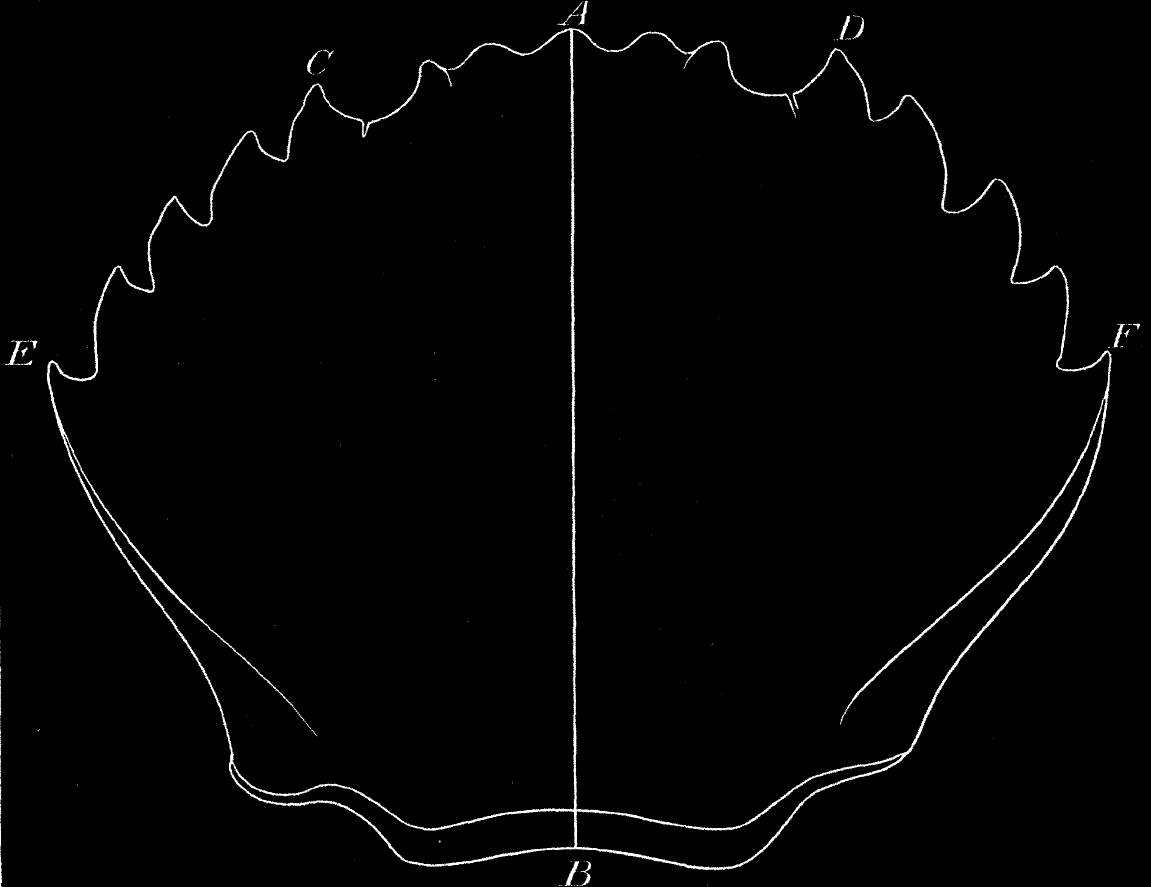
\includegraphics[width=6cm]{images/crabe.png}
		\end{center}
		\label{fig:crabe}
	\end{figure}
\end{frame}

\begin{frame}{}
	\begin{columns}
		\column{.4\textwidth}
	\begin{figure}[hbp]
		\begin{center}
			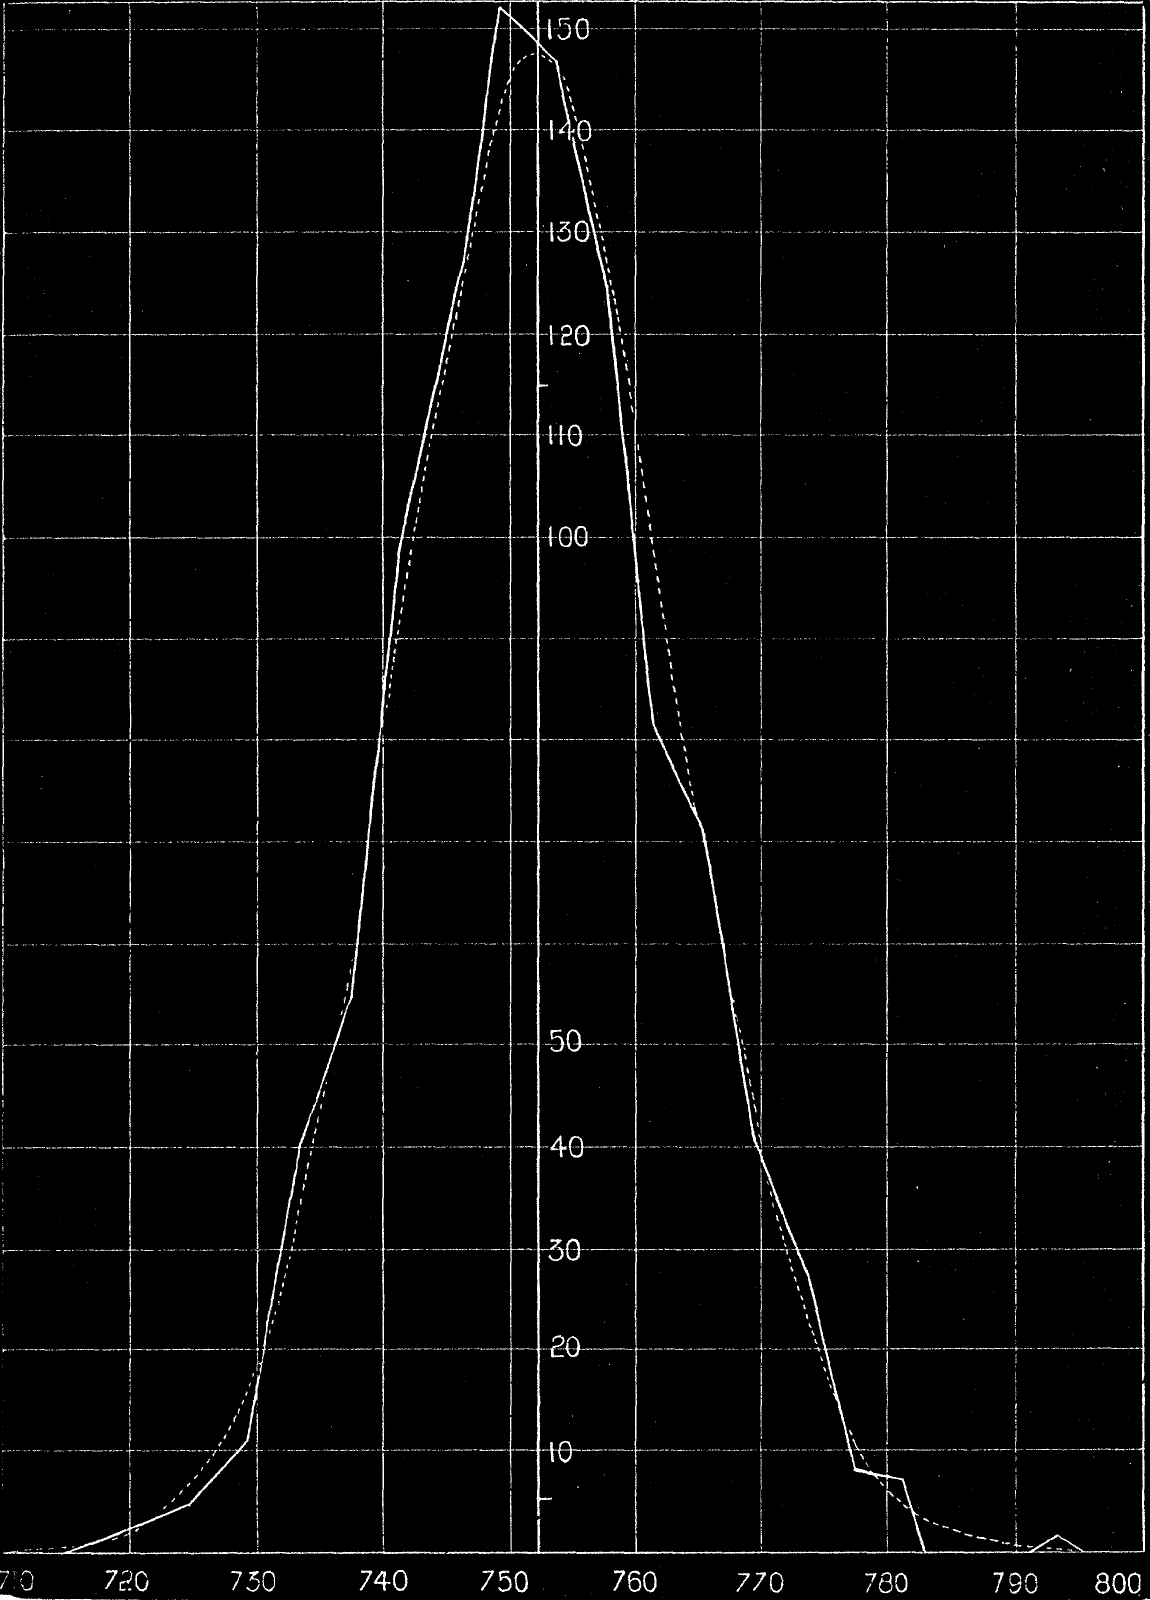
\includegraphics[width=4cm]{images/gauss1.png}
		\end{center}
	\end{figure}

	\column{.6\textwidth}

	\begin{figure}[hbp]
		\begin{center}
			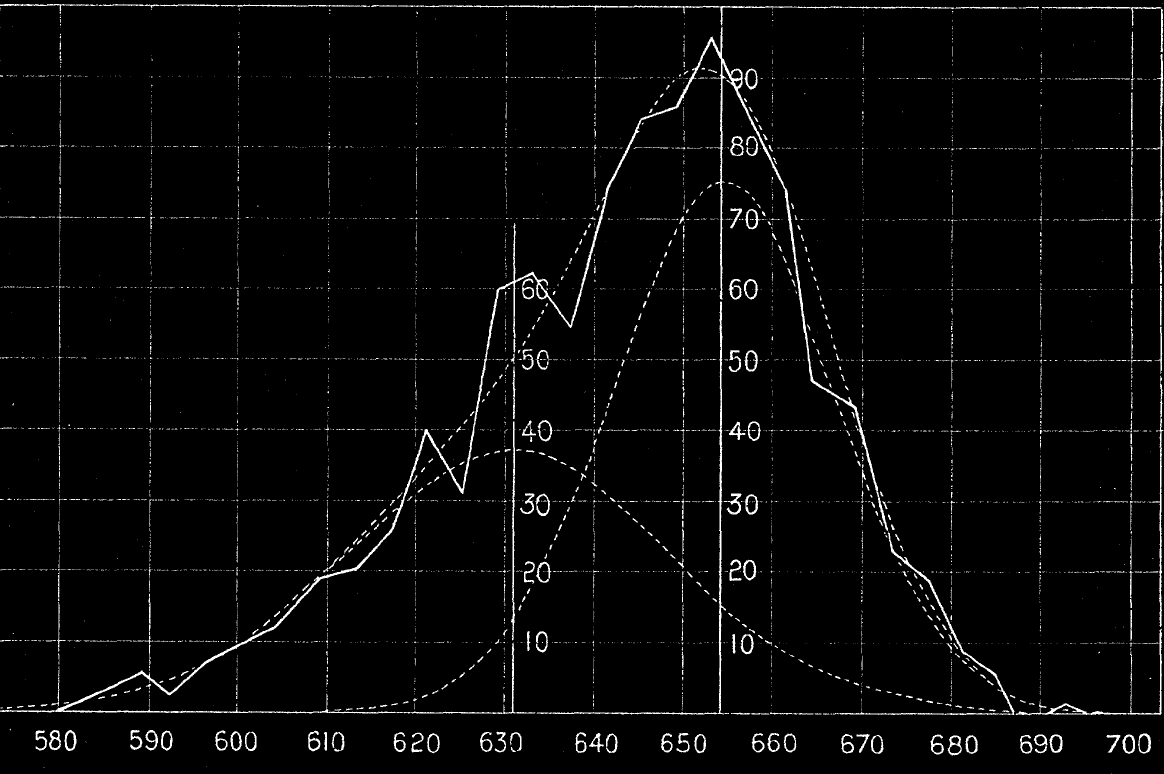
\includegraphics[width=6cm]{images/gauss2.png}
		\end{center}
	\end{figure}
\end{columns}
\begin{center}
	(from Weldon 1893)
\end{center}

\end{frame}


\subsection{Mendelism}
\begin{frame}{Mendelism}
	Beggining of XXe : rediscovery of Mendel's works (by de Vries):
	\vfill
	\begin{itemize}
		\item no continu variations,
		\item hybridation of discontinuous traits 
		\item evolution : jump \& large mutation (saltationism)
	\end{itemize}
	\vfill

	In contradiction with Darwin:

	$\rightarrow$ species appear with large mutations, by ``jumps'' : not by the action of Natural Selection .

	
\end{frame}



\begin{frame}{Modern Synthesis}
	Reconciliate Mendel \& Darwin through the genetc theory of evolution Fisher 1918, Haldane \& Wright.\\

	$\rightarrow$ Population genetics.
	\vfill 

	Even between actor some vision are differents :
	\begin{itemize}
		\item Fisher : Newton-like ideal  ``the Fundamental Theorem of Natural Selection''.
		\item Wright : local adaptation : the model of ``Adaptative Landscapes''.
	\end{itemize}

	\begin{columns}
	\column{.5\textwidth}
		\begin{figure}[hbp]
			\begin{center}
				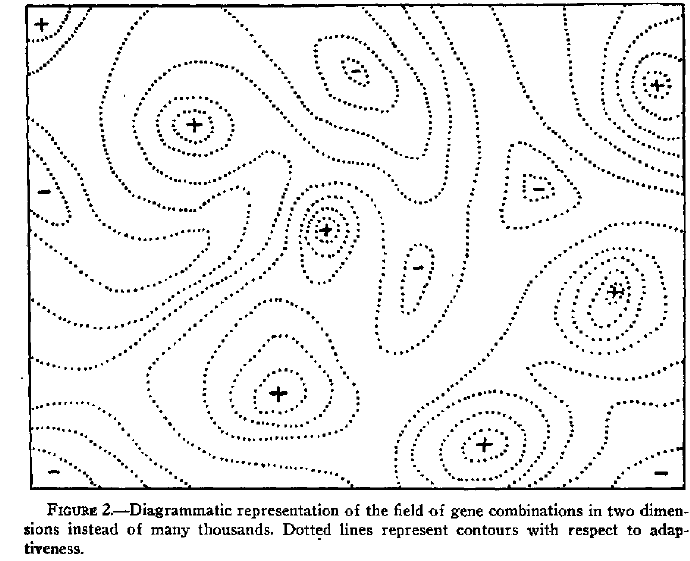
\includegraphics[width=4cm]{images/wrightFL.png}
			\end{center}
		\end{figure}
	\column{.5\textwidth}
		\begin{figure}[hbp]
			\begin{center}
				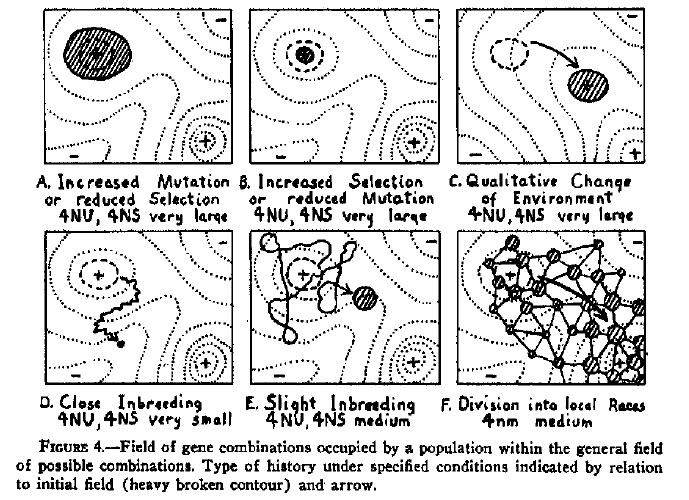
\includegraphics[width=5cm]{images/wrightFL2.png}
			\end{center}
		\end{figure}
	\end{columns}

	\vfill
	Years of synthesis : all biological related domains are rattached to the genetec theory of evolution (30's 60's).

\end{frame}

\subsection{Modern Synthesis}
\begin{frame}{An evolutionary synthesis}
	Modern synthesis, emergence of a consensus
	\begin{itemize}

		\item	Biological individual are the product of genetical information transmitted by the germ line (Followin Weisman and central dogma):

			\begin{center}
				DNA$\rightarrow$transcription$\rightarrow$traduction$\rightarrow$protein
			\end{center}

		\item Genetical information spread from $G^-$ to $G^-$ via DNA which randomly vary.

	\item Evolution is change in allele frequencies. 

	\end{itemize}


\end{frame}


\section{Nowaday issus}
\subsection{Level and unit of selection}
\begin{frame}{Level and unit of selection}

	Lewontin (1972):
	\vfill
	In a population,
	\begin{enumerate}
		\item indiv. $\ne$ $\rightarrow$ morpho., physio., behavior $\ne$ (\alert{phenotypic variation}).
		\item phenotypes $\ne$ $\rightarrow$ survival or reproductive rates $\ne$ in $\ne$ env. (\alert{differential fitness}).
		\item correlation btw parents \& offsprints each $G^-$ futur (\alert{fitness heredity}).
	\end{enumerate}
	\vfill

	This definition don't impose a level of biological organisation. 
	
	So which one is the right one? (gene, chromosomes, organism, organes, species\ldots)?
\end{frame}

\begin{frame}{Level \& Unit of selection}
	Different approach of the pb (Gould : human cognitive limitation) 
	\vfill
	\begin{itemize}
		\item Hull-Dawkins : replicator/interactor. 
		\item Superorganism (Wilson \& Sober).
		\item \ldots
	\end{itemize}


	Questions that have to be answered when applying Darwin to Musical structures.

\end{frame}

\subsection{Population darwinienne}
\begin{frame}{Godfrey-Smith, darwinian population}
	Peter Godfrey-Smith thinks that ``recipes'' have problems
	\vfil
	\begin{itemize}
		\item Mix to hardly councilable goals : 
			\begin{itemize}
				\item  ``Universal''algorithm
				\item Be able to describe eveyr evolutives tales.
			\end{itemize}
	\end{itemize}
	\vfill
	It's impossible, so:
	$\rightarrow$  Darwinian Population 
	\begin{enumerate}
		\item Minimals (Lewontin's recipes)
		\item Paradigmatics (clear multicell. orga.  w/ sexual reproduction (Darwin analogy)  \ldots )
		\item Marginals
	\end{enumerate}
	
\end{frame}

\begin{frame}{PGS' space}
	%Partant des propriétés nécessaires aux populations minimales il extrait un ensemble de propriétés:
	%\begin{itemize}
	%	\item H : Fidélité de l'hérédité.
	%	\item V : Abondance variation.
	%	\item $\alpha$ : Interaction compétitive vis à vis reproduction.
	%	\item S : Dépendance de la reproduction différentiée à des facteurs internes.
	%	\item C : Continuité, régularité du paysage adaptatif.
	%\end{itemize}
	%\vfil
	
	\begin{figure}[h]
		\begin{center}
			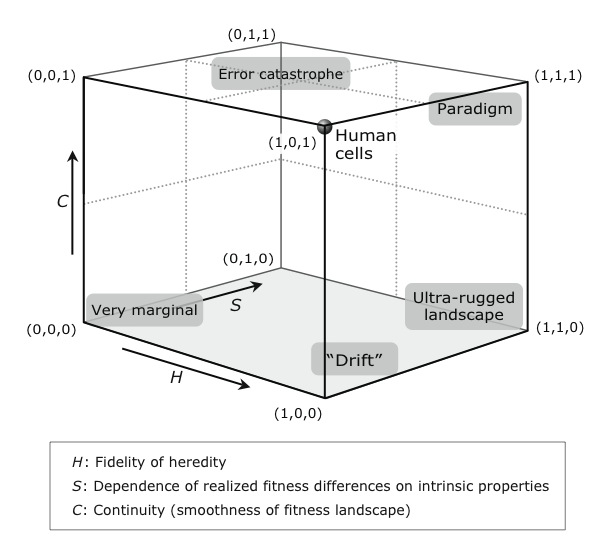
\includegraphics[width=5cm]{./images/PGS.png}
		\end{center}
		\caption{from PGS (2009, p.64)}
		\label{fig:PGS}
	\end{figure}
	
	Decomposition into sub properties, ideal frame to include radically differents objects.
\end{frame}

\section{Conclusion}
	
\begin{frame}{Conclusion}
	The questions handeled by darwinian theory of evolution are huge and complexes. 
	Export the theory out of is orginal bounds can be valuable for many reasons but one have always to keep in mind \emph{what} he is trying to use and \emph{how} he will use it.
		
\end{frame}


\end{document}
